\chapter{The 6LoWPAN Implementation - BLIP/TinyOS}
\label{Blip/TinyOS}
As mentioned in Section \ref{Intr:Motiv}, there are several implementations for 6LoWPAN, such as uIPv6, BLIP, Sensinode's NanoStack, Jennic's 6LoWPAN and Nivis ISA100.11a. Among all those implementations, BLIP for TinyOS is well known and respected due to its many useful applications. Using BLIP/TinyOS, one is able to form multi-hop IP networks consisting of different nodes communicating over shared protocols \cite{BLIP}. Simulation of BLIP/TinyOS is the main focus of the research of this paper.

\section{TinyOS}
\label{TinyOS}
TinyOS is a light-weight open source operating system designed for low-power wireless devices, such as those used in sensor networks, ubiquitous computing, personal area networks, smart buildings, and smart meters \cite{TinyOS}. It allows for various applications to be installed on sensor nodes via USB connections. The language that is used in TinyOS is NesC, which is a dialect of the C language. NesC is a component-based as well as event-driven programming language; the components are wired together using interfaces. NesC was designed to make the operating system optimized for the memory constraints of sensors.

The latest official release is TinyOS 2.1.1. It supports multiple platforms, such as Mica-family, Telos-family, epic, mulle, and shimmer2 platforms. 

\subsection{Radio Stack}
\label{Sim:radio stack}
\begin{figure}[htbp]
  \begin{center}
    \leavevmode
      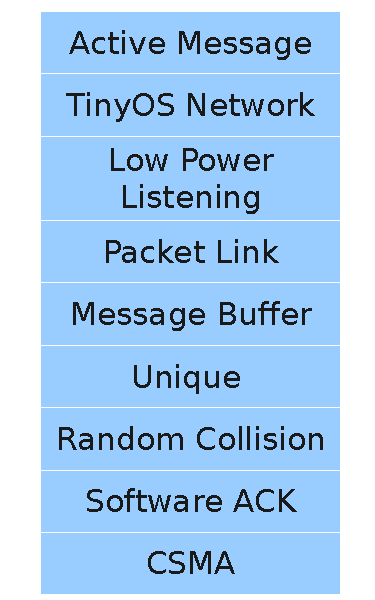
\includegraphics[scale=0.5]{Pics/Rfxlinklayer.pdf}
   \caption{Radio stack for rfxlink}
    \label{fig:rfxlinklayer}
  \end{center}
\end{figure}
\index{figure 4.1}
Different platforms might use different radio chips. For example: Micaz platforms use CC2420 and TelosB, and IRIS uses RF230. Most of the low-level transmission and receiving packets are taken care of by the radio chip hardware, specifying the proper behavior of that hardware requires a well defined radio stack implementation \cite{TEP 126}. 
An new radio stack called rfxlink is added in TinyOS 2.1.1. The rfxlink stack unifies CC2420 and RF230 software radio stacks, and only leaves chip driver part different. It is the future standard radio stack. In addition, TOSSIM support has been added to the rfxlink stack.
The rfxlink radio stack includes several layers which are shown in Figure \ref{fig:rfxlinklayer}. 
\section{The implementation - BLIP}
\label{Blip}
BLIP, short for the Berkeley Low-power IP stack, is an implementation of 6LoWPAN adaptation layer and IP layer. It was included as a core part of TinyOS. The main parts of the BLIP implementation consist of:
\begin{itemize}
\item Transport layer: BLIP implements User Datagram Protocol (UDP), Transmission Control Protocol (TCP) and Internet Control Message Protocol (ICMP) in this layer.

\item Network layer: in this layer, BLIP defines the routing protocol for Low power and Lossy Networks (LLNs), such as HYDRO or RPL.
 
\item 6LoWPAN adaptation layer: as mentioned in Section \ref{Intr:6LoWPAN}, this layer compress certain higher-level headers and break large packets into multiple link-layer fragments.
\end{itemize}

BLIP has changed considerably since BLIP version 1.0. In May 2010, BLIP version 2.0 has been added to the TinyOS repository. 
\subsection{Difference between BLIP 1.0 and BLIP 2.0}
\label{Blip:1.0-2.0}

\begin{figure}[htbp]
  \begin{center}
    \leavevmode
    %\framebox{
    \subfloat[BLIP 1.0]{\label{fig:blip1.0}
      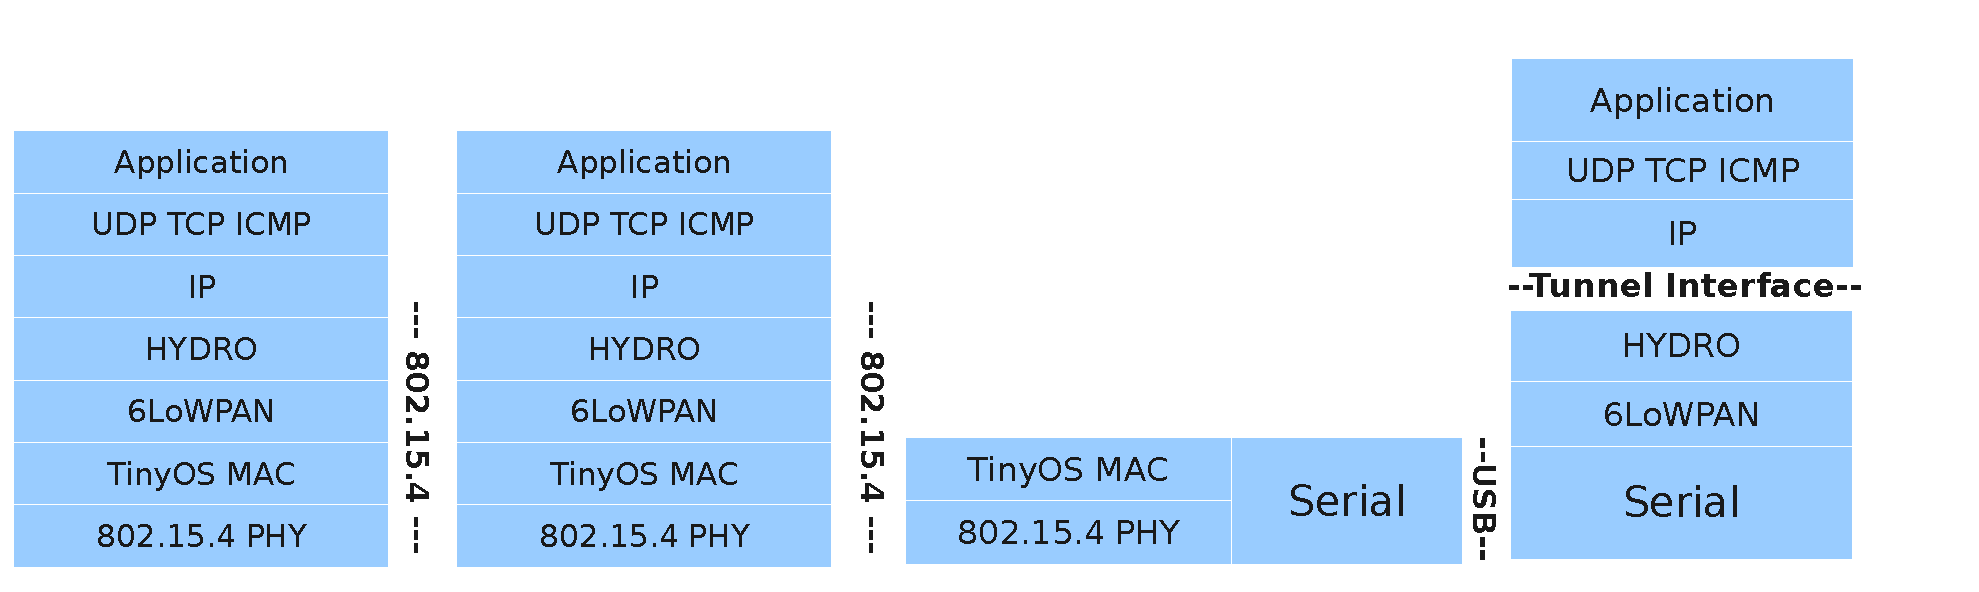
\includegraphics[scale=0.4]{Pics/blip1.pdf}}\\
    \subfloat[BLIP 2.0]{\label{fig:blip2.0}
       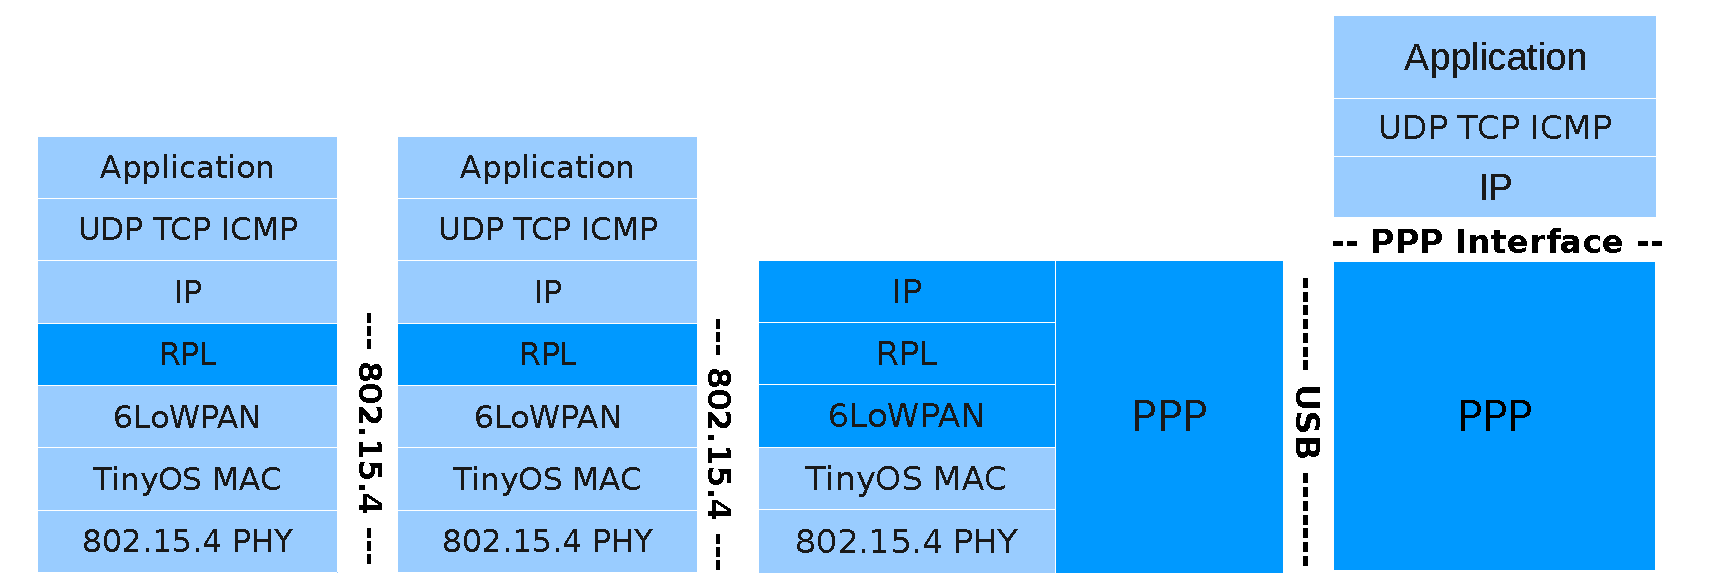
\includegraphics[scale=0.4]{Pics/blip2.pdf}}
    \caption{Protocol stacks for BLIP}
    \label{fig:blip}
  \end{center}
\end{figure}

An overview of the protocol stack for both BLIP implementations can be found in Figure~\ref{fig:blip}. BLIP 2.0 introduces RPL instead of HYDRO as the routing protocol. Compared to HYDRO, RPL employs a more sophisticated way to discover topological changes and react accordingly. Moreover, RPL is more standard compliant than HYDRO.

The second main change is in the border router. Version 2.0 employs an IP layer router with a Point-to-Point Protocol (PPP) interface. The PPP interface provides a PPP connection to a normal IP device, which can then perform some higher level functionalities such as request data or give instructions.

Since BLIP 1.0 was updated to BLIP 2.0, the simulation of BLIP had to be re-enabled as well. The next chapter gives details about the simulation, including information about the simulator, how the simulation was enabled, and the scenario setups.

